
\section{Muon System}

Muons at CMS~\cite{muon_tdr} are measured in the pseudorapidity range $\abs{\eta} < 2.4$, with detection planes made using three technologies: drift tubes, cathode strip chambers, and resistive plate chambers, as presented in Figure~\ref{cms_muon}. The single muon trigger efficiency exceeds 90\% over the full $\eta$ range, and the efficiency to reconstruct and identify muons is greater than 96\%. Matching muons to tracks measured in the silicon tracker results in a relative transverse momentum resolution, for muons with \pt up to 100\GeV, of 1\% in the barrel and 3\% in the endcaps. The \pt resolution in the barrel is better than 7\% for muons with \pt up to 1\TeV~\cite{Sirunyan:2018}. 

% cms muon
\begin{figure}[htbp]
    \centering
    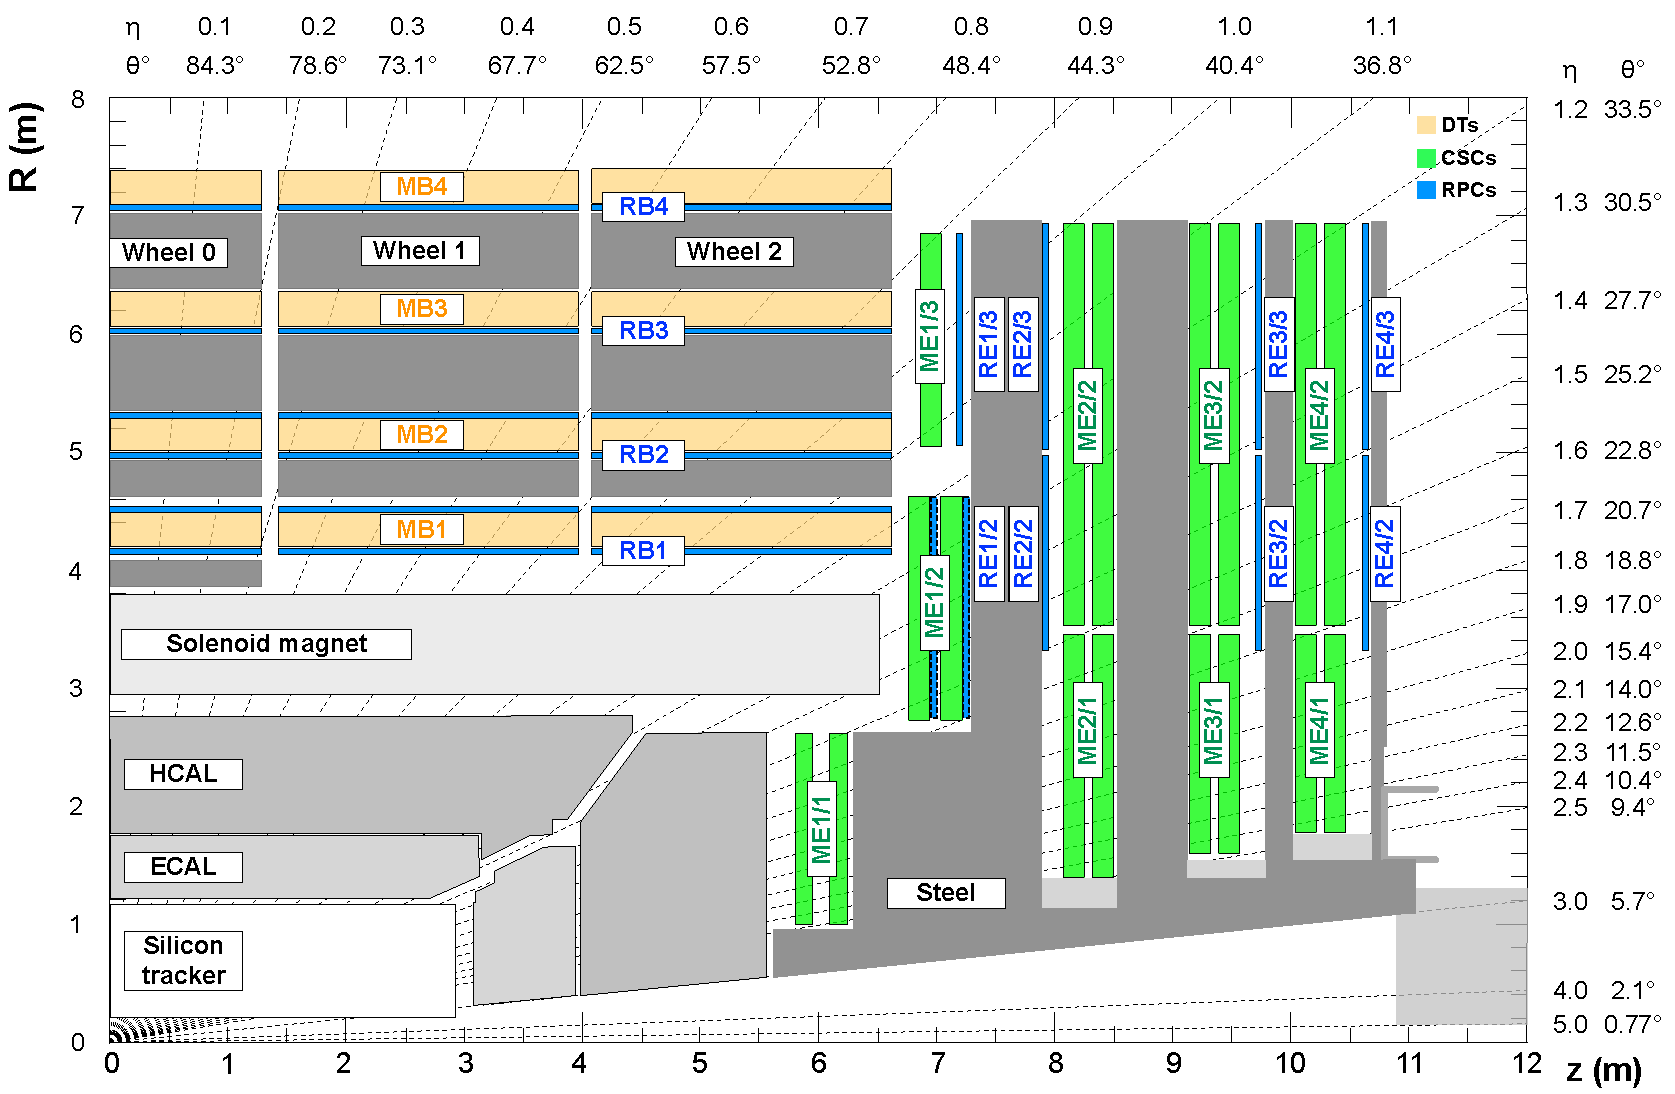
\includegraphics[width=\textwidth]{figures_and_tables/experimental_setup/cms_muon.pdf}
    \caption{Longitudinal section view of the ECAL and its components. Source:~\cite{Chatrchyan:2013sba}.}
    \label{cms_muon}
\end{figure}

The muon detection system has around 1 million channels. For Run3, the muon system is being expanded and upgraded, by the inclusion of new chamber with the Gas Electron Multiplier (GEM)~\cite{Sauli:2262884} technology.

\subsection{Drift Tubes}

The Drift Tubes (DT)~\cite{Teyssier:2015xjj} are gaseous detectors (85\% Ar and 15\% CO2) installed in the central region of CMS (Barrel - blue regions at Figure~\ref{cms_muon}), covering the region of $|\eta < 1.2|$. The barrel is divided in 5 wheels, along $z$, W+2, W+1, W0, W-1 and W-2. Each will is composed by four concentric stations along $r$, MB 1 to MB4, and each station is divided in 12 sectors along $\phi$, S01 to S12. In total, there are 205 DT chambers. Each tube has 50 $\mu$m tick (diameter) gold-plated stainless steel wire, as well as, kept at positive voltage, and aluminum electrodes. The signal is read on the golden wire only.

The tubes are arranged in layers and occupy the whole length of the chamber. The tubes are arranged in coaxial layers. Each set of three layers, forms a Super-Layer (SL).The first and the last SL are aligned in the, so called, $r-\phi$ direction, while the middle one, in the $r-z$ direction, transversal to the previous one. This arrangement give the DTs, the possibility to measure the passage of a muon in $\eta$ and $\phi$ direction, with a resolution of 100 $\mu$m.

